\chapter{Versuchsaufbau und Messprinzip}
Im Gegensatz zum Interferometer von Albert Abraham Michelson und Edward Williams Morley macht der Versuch sich nicht die
Eigenschaft des Lichtes zu interferieren zu nutze, sondern misst Laufzeitunterschiede kurzer Lichtpulse.\par
Der optische Aufbau ist allerdings sehr ähnlich. Ein Lichtpuls verlässt eine Lichtquelle und wird an einem Strahlteiler - 
ein halbdurchlässiger Spiegel angeordnet im Winkel von \(45\degree\) zur optischen Achse - in zwei Teilstrahlen zerlegt.
Ein Teilstrahl wird hierbei in die Photodiode A umgelenkt. Die Bewegungsrichtung unverändert passiert der übrige Strahl
eine \textsc{Fresnel}-Linse, wird an einem Prismen-Reflektor zurückgeworfen, passiert abermals die \textsc{Fresnel}-Linse und wird schließlich
am Strahlteiler in eine zweite Photodiode B abgelenkt (vgl. \bild{fig:strahlteilung}).\par
%
\begin{figure}[h]
    \centering
    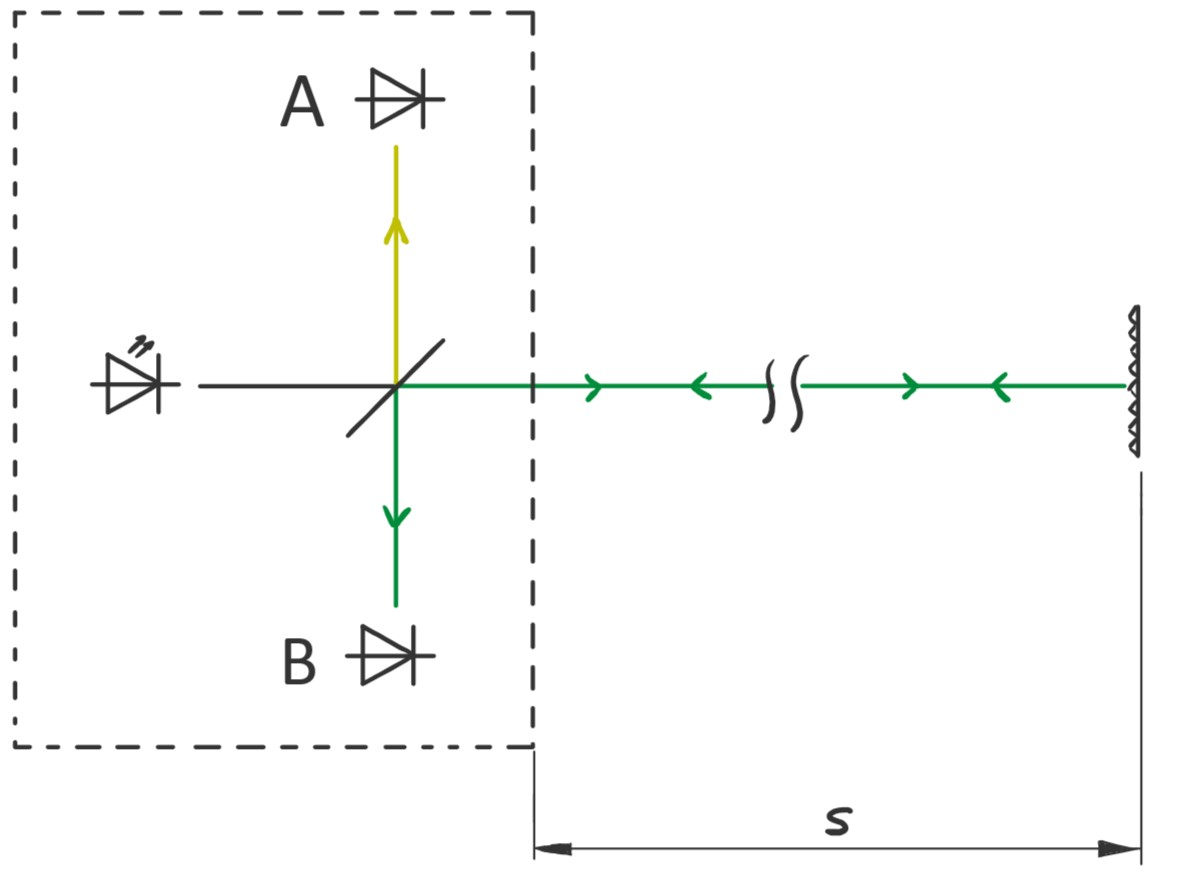
\includegraphics[width=.6\textwidth]{aufbau/strahlteilung.jpg}
    \caption[Skizze der Strahlgänge]{Skizze der Strahlgänge mit den Photodioden A und B. Gemessen wird die Strecke \(s\) vom Ausgang der Pulsquelle bis zum Prismen-Reflektor.}
    \label{fig:strahlteilung}
\end{figure}
%
\begin{figure}[h]
    \centering
    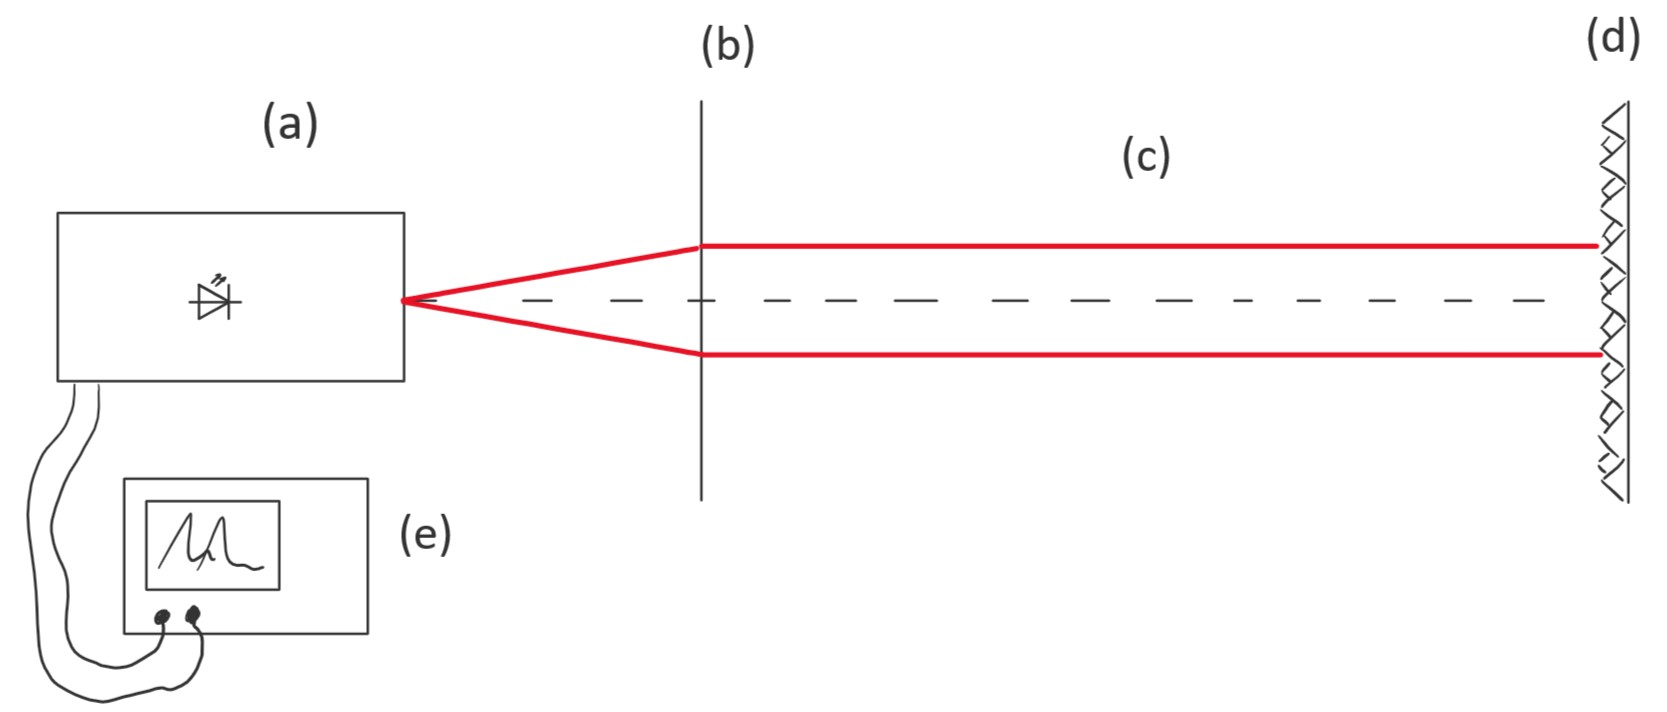
\includegraphics[width=.9\textwidth]{aufbau/devices.jpg}
    \caption[Anordnung der verwendeten Geräte]{Anordnung der verwendeten Geräte: (a) Pulsquelle mit Strahlteiler und Photodioden (b) \textsc{Fresnel}-Linse (c) Lichtstrahl (d) Prismen-Reflektor (e) Oszilloskop.}
    \label{fig:devices}
\end{figure}
%
Der in Photodiode A erzeugt Puls dient als Referenzimpuls. Da Licht keine instantane also endliche Wirkgeschwindigkeit
hat ist der in Photodiode B erwartete Puls durch die größere zurückgelegte Strecke gegenüber dem Referenzimpuls um die
Zeitdifferenz \(\Delta t\) phasenverschoben. Diese Differenz ist durch
\begin{equation}
    \Delta t = \frac{1}{c} \Delta s
\end{equation}
proportional zur Streckenänderung \(\Delta s\) mit \(c^{-1}\) als Proportionalitätsfaktor. Das erwartete Oszillogram ist
in \bild{fig:puls_skizze} dargestellt.\par
\begin{figure}[h]
    \centering
    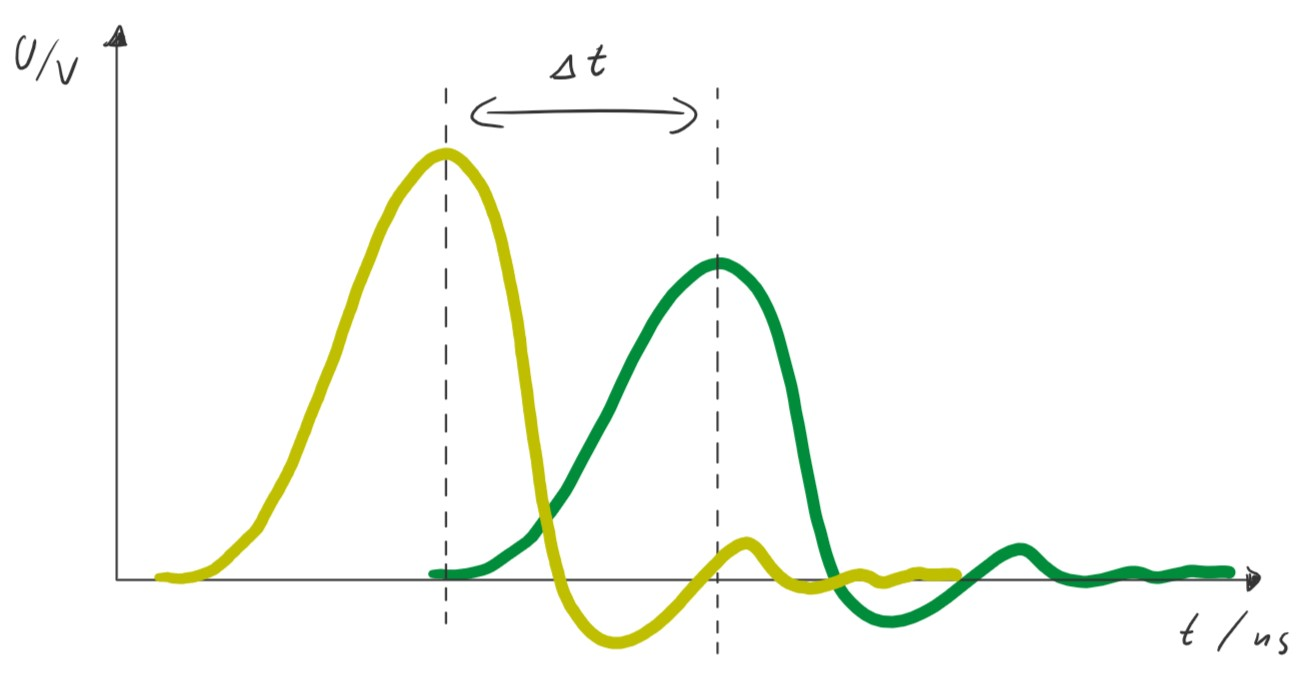
\includegraphics[width=.9\textwidth]{aufbau/signal_skizze_wht.jpg}
    \caption[Schematische Darstellung des erwarteten Oszillograms]{Schematische Darstellung des erwarteten Oszillograms.
            Referenzpuls in gelb und der um \(\Delta t\) phasenverschobene Puls des Messsignals in grün. Durch Streuung und
            Intensitätsverluste in den optischen Medien ist die Amplitude des Messignals um \(\Delta U\) geringer. Dies
            ist für den Versuch allerdings irrelevant.}
    \label{fig:puls_skizze}
\end{figure}